\documentclass{article}
\usepackage[utf8]{inputenc}
\usepackage{minted}
\usepackage[a4paper, top=1in, left=0.5in, right=0.5in, bottom=1in]{geometry}
\usepackage{fancyhdr}
\usepackage{tikz}
\usepackage{pgfplots}
\usepackage{amssymb}

\setcounter{secnumdepth}{5}
\setcounter{tocdepth}{5}
\pgfkeys{/pgf/number format/.cd,1000 sep={\,}}

\pagestyle{fancy}
\chead{\Large{Reference document, Nikolay Budin}}
\lhead{Generated \today \\
\textcolor{red}{1 error}, \textcolor{orange}{1 warning}
}
\rhead{ITMO University}

\begin{document}
\tableofcontents

\newpage

\section{String algorithms}
\subsection{Manacher algorithm (longest palindrome for every center)}
\inputminted[mathescape, breaklines, tabsize=4]{c++}{./strings/manacher/manacher.cpp}
\checkmark Tests passed
\begin{center}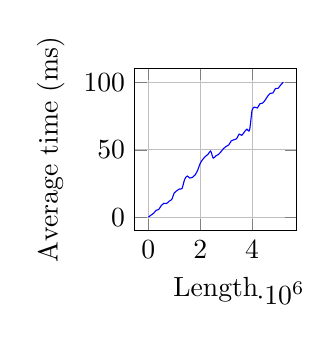
\begin{tikzpicture}
	\begin{axis}[
		xlabel=Length,
		ylabel=Average time (ms),
		grid=major,
		scaled y ticks=false,
		y tick label style={/pgf/number format/fixed},
		width=0.3\textwidth,
		height=0.3\textwidth]
	\addplot[color=blue, smooth] coordinates {
		(1, 0.00005)
(100001, 1.40368)
(200001, 2.80980)
(300001, 5.01359)
(400001, 5.68073)
(500001, 8.67425)
(600001, 10.27697)
(700001, 10.10974)
(800001, 11.78291)
(900001, 13.05420)
(1000001, 18.02830)
(1100001, 19.68207)
(1200001, 20.98612)
(1300001, 21.33491)
(1400001, 28.13082)
(1500001, 30.54476)
(1600001, 29.00368)
(1700001, 29.62417)
(1800001, 31.31427)
(1900001, 34.82401)
(2000001, 40.01716)
(2100001, 43.01713)
(2200001, 45.19695)
(2300001, 46.70973)
(2400001, 49.11350)
(2500001, 43.93777)
(2600001, 45.52613)
(2700001, 46.63391)
(2800001, 48.62473)
(2900001, 51.04052)
(3000001, 52.62166)
(3100001, 53.75703)
(3200001, 56.78241)
(3300001, 57.58574)
(3400001, 58.26005)
(3500001, 61.76028)
(3600001, 60.85257)
(3700001, 63.34761)
(3800001, 65.45987)
(3900001, 64.73827)
(4000001, 79.67618)
(4100001, 81.81411)
(4200001, 81.19081)
(4300001, 84.33990)
(4400001, 84.80905)
(4500001, 87.02352)
(4600001, 90.03197)
(4700001, 92.09755)
(4800001, 92.34361)
(4900001, 95.67335)
(5000001, 95.84056)
(5100001, 98.34652)
(5200001, 100.41516)

	};
	\end{axis}
\end{tikzpicture}\end{center}\subsection{Prefix function}
\inputminted[mathescape, breaklines, tabsize=4]{c++}{./strings/pref_function/pref_function.cpp}
\checkmark Tests passed
\begin{center}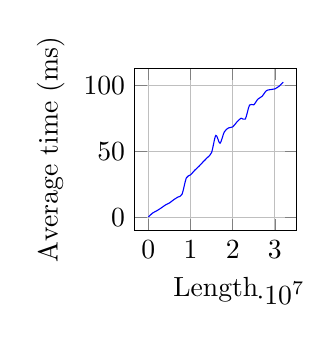
\begin{tikzpicture}
	\begin{axis}[
		xlabel=Length,
		ylabel=Average time (ms),
		grid=major,
		scaled y ticks=false,
		y tick label style={/pgf/number format/fixed},
		width=0.3\textwidth,
		height=0.3\textwidth]
	\addplot[color=blue, smooth] coordinates {
		(1, 0.00004)
(1000001, 3.04782)
(2000001, 4.79016)
(3000001, 6.82951)
(4000001, 9.09451)
(5000001, 10.70848)
(6000001, 13.16447)
(7000001, 15.19880)
(8000001, 17.39937)
(9000001, 29.70328)
(10000001, 32.05185)
(11000001, 35.57767)
(12000001, 38.58729)
(13000001, 42.00489)
(14000001, 45.22427)
(15000001, 49.05340)
(16000001, 62.04580)
(17000001, 56.10121)
(18000001, 64.61456)
(19000001, 67.72562)
(20000001, 68.48828)
(21000001, 72.24345)
(22000001, 75.13236)
(23000001, 74.47957)
(24000001, 85.12094)
(25000001, 85.28631)
(26000001, 89.67687)
(27000001, 91.81448)
(28000001, 96.06844)
(29000001, 96.84945)
(30000001, 97.39997)
(31000001, 99.42471)
(32000001, 102.50109)

	};
	\end{axis}
\end{tikzpicture}\end{center}\subsection{Suffix structures}
\subsubsection{Suffix array}
\inputminted[mathescape, breaklines, tabsize=4]{c++}{./strings/suff_algorithms/suff_array/suff_array.cpp}
\checkmark Tests passed
\begin{center}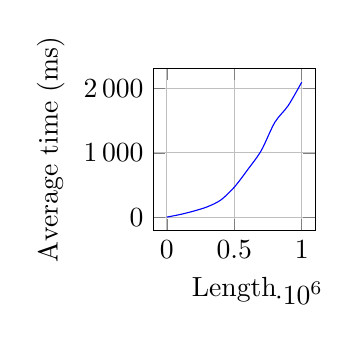
\begin{tikzpicture}
	\begin{axis}[
		xlabel=Length,
		ylabel=Average time (ms),
		grid=major,
		scaled y ticks=false,
		y tick label style={/pgf/number format/fixed},
		width=0.3\textwidth,
		height=0.3\textwidth]
	\addplot[color=blue, smooth] coordinates {
		(1, 0.00047)
(100001, 40.81160)
(200001, 93.77239)
(300001, 159.74959)
(400001, 265.18201)
(500001, 465.04838)
(600001, 739.25857)
(700001, 1034.47205)
(800001, 1472.12715)
(900001, 1735.42908)
(1000000, 2099.11813)

	};
	\end{axis}
\end{tikzpicture}\end{center}\section{FFT}
\subsection{FFT by modulo}
\inputminted[mathescape, breaklines, tabsize=4]{c++}{./fft/mod/mod_fft.cpp}
\textcolor{red}{\textbf{Error:} Compilation error while compiling test}
\subsection{FFT in complex numbers}
\textcolor{orange}{\textbf{Warning:} Leaf directory without any information}


\end{document}
